% -*- TeX-engine: default; fill-column: 80; -*-
\documentclass[sigconf]{acmart}
\usepackage[font=footnotesize]{subcaption}
\usepackage[utf8]{inputenc}
\usepackage[T1]{fontenc}
\usepackage{url}
\usepackage{booktabs}
\usepackage{xcolor}

\setcopyright{ccbysa}
\acmConference[LPC '18 Networking Track]{Linux Plumbers Conference 2018 Networking Track}{Nov 13--14,
2018}{Vancouver, British Columbia}
\acmISBN{}
\acmDOI{}
\settopmatter{printccs=false, printacmref=false}
%\widowpenalty=100
%\clubpenalty=100
%\brokenpenalty=100

\begin{document}
\title{XDP -- challenges and future work}
\author{Jesper Dangaard Brouer}
\affiliation{%
  \institution{Red Hat}}
\email{brouer@redhat.com}

\author{Toke Høiland-Jørgensen}
\affiliation{%
  \institution{Karlstad University}}
\email{toke@toke.dk}


\captionsetup{font+=small}


\begin{abstract}
  XDP continues to see significant development, and is far from a finished
  system. However, XDP already offers rich facilities for high performance
  packet processing, and has seen deployment in several production systems.

  In this work, we provide an overview over some of the ongoing work around XDP,
  and seek to start a discussion on some of the future challenges that need to
  be addressed to make sure the XDP ecosystem can continue to flourish.

  The overview of ongoing work focuses on the XDP-related topics being discussed
  at the LPC networking track in Vancouver, where we provide a short overview of
  each topic, and refer to the talk for more details. These topics include
  production deployment reports, using XDP as a backend for the P4 language,
  zero-copy to userspace with AF\_XDP, and the use of kernel helpers to evolve
  the XDP feature set. We also include some performance numbers from the
  academic paper on XDP that we have co-authored with many of the other XDP
  developers.

  In the forward-looking section, we discuss some future developments that we
  believe would be beneficial to work on going forward. These topics include NIC
  memory models and DMA mapping; moving SKB allocation out of drivers; the
  resource allocation around ndo\_xdp\_xmit; whether it is still realistic to
  aim for full support of all XDP features in all drivers; and the possibility
  for adding an XDP egress hook. We are hoping to solicit feedback on these from
  the wider community during and after LPC.
\end{abstract}


\maketitle

\section{Introduction}%
\label{sec:introduction}

We have recently finished writing an academic paper on XDP~\cite{xdp-paper},
which includes a description of the architecture, and performance comparison
with DPDK. As part of that work, we have discussed several areas of potential
improvements to XDP as a whole. The purpose of this paper, and the associated
talk, is to broaden that discussion to the wider community, and to solicit
feedback on some of the future directions we see as beneficial for XDP.

To provide some context to the discussion of future directions, we first look at
some of the work that is currently ongoing. We do this in the form of an
overview of the other XDP-related talk and topics that will be covered at the
networking track at LPC\,'18. Those topics will not be covered in detail in this
work, but we provide a short summary of each, with references to the other
talks. This is the topic of Section~\ref{sec:current}.

Following this, we discuss some possible future developments that we believe
will be beneficial to XDP's development going forward. This is the topic of
Section~\ref{sec:future}, and takes the form of a short summary of each
development, which should be seen more as an invitation to provide feedback than
a finished roadmap.

\section{Current developments around XDP}
\label{sec:current}

Even though XDP is still being very actively developed (as the large number of
talks at LPC shows), we have already seen examples of it being successfully
deployed in production environments. High-profile examples include Cloudflare's
use for DDOS protection~\cite{cloudflare-ddos}, and Facebook's Katran load
balancer~\cite{katran}. There are also XDP plugins for Suricata~\cite{suricata},
Open vSwitch~\cite{ovs-xdp}, and even DPDK~\cite{dpdk-xdp}.

There are two other talks at LPC that cover Facebook's production use of XDP in
more detail~\cite{facebook-lessons,facebook-firewall}.

In this section we seek to give an overview of the current state of XDP and some
of the ongoing development that is being presented at LPC.

\subsection{The state of XDP performance}
\label{sec:state-xdp-perf}

XDP has been deliberately designed to achieve maximum packet processing
performance. This is achieved by combining several techniques, such as avoiding
memory allocations in the processing path, and running the processing at the
earliest possible time after packets are received from the hardware. The results
of these efforts is the impressive performance shown in
Figures~\ref{fig:drop-test} and \ref{fig:redirect-test} (both from the XDP
paper~\cite{xdp-paper}).

\begin{figure}[t]
\centering
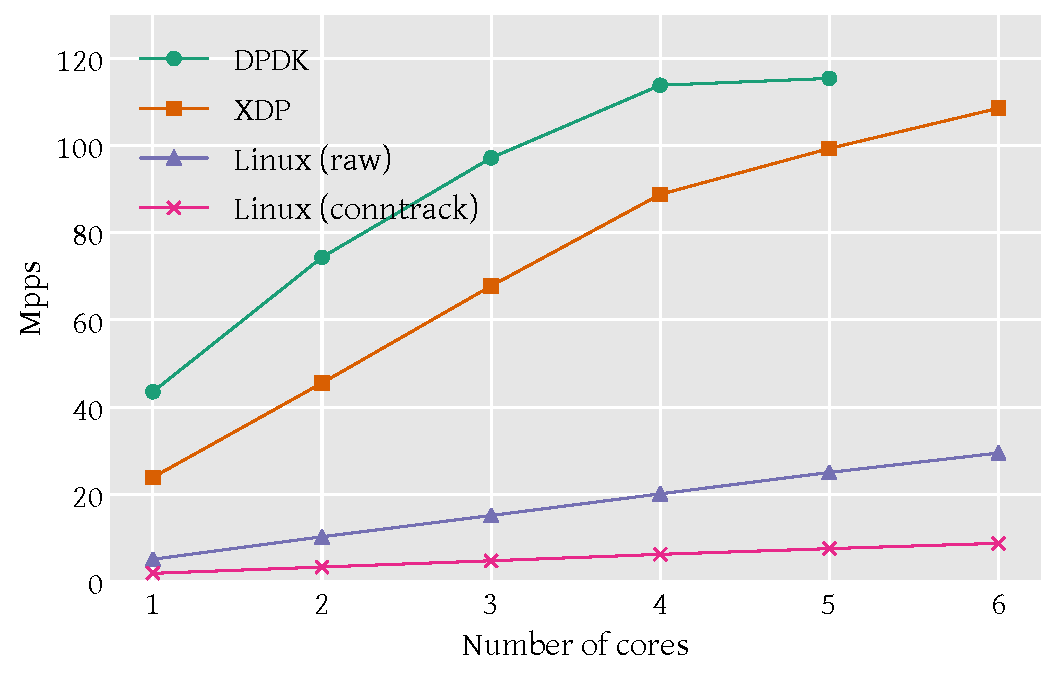
\includegraphics[width=\linewidth]{images/drop-test.pdf}
\caption{\label{fig:drop-test} Packet drop performance. DPDK uses one core for
  control tasks, so only 5 are available for packet processing.}
\end{figure}

\begin{figure}[t]
\centering
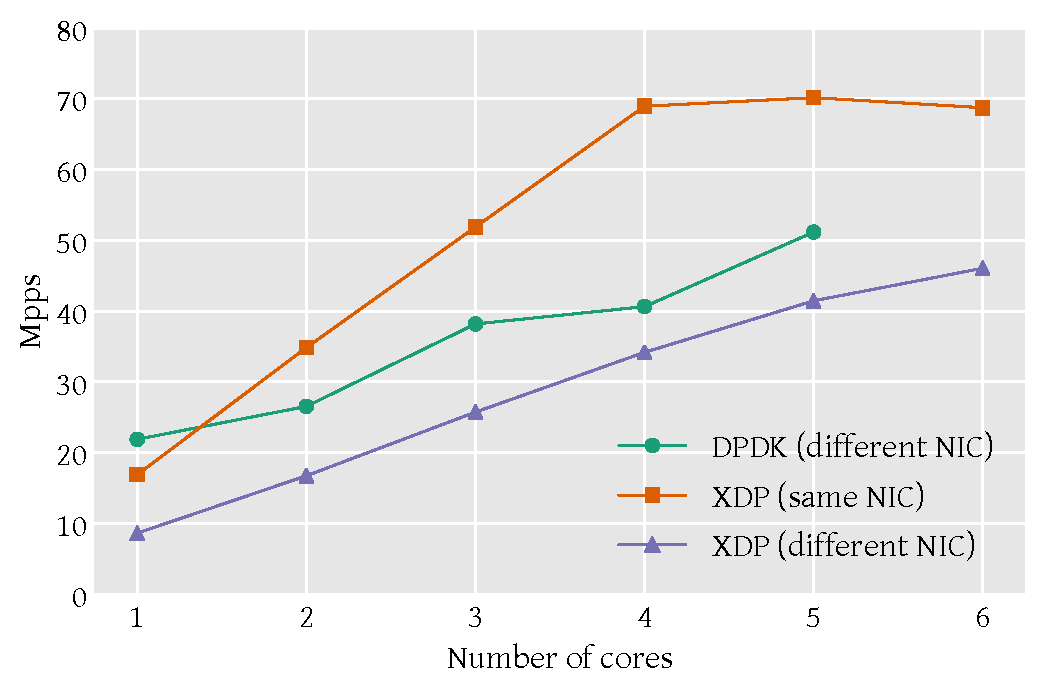
\includegraphics[width=\linewidth]{images/redirect-test.pdf}
\caption{\label{fig:redirect-test} Packet forwarding throughput. Sending and
  receiving on the same interface takes up more bandwidth on the same PCI port,
  which means we hit the PCI bus limit at 70 Mpps.}
\end{figure}

However, attaining this level of performance is not trivial, and the smallest
optimisations (or conversely, small additions of overhead) can have a large
impact. As an example, the Mellanox driver we used for our tests
(\texttt{mlx5}), performs 10 non-inlined function calls for every packet. Our
tests show that the overhead \emph{of just the function calls} corresponds to an
additional 9\,Mpps of performance on a single core.

% Should we mention that some of the non-inlined mlx5 driver function
% calls are indirect function pointer calls?  Which will be even worse
% when enabling CONFIG_RETPOLINE. But that is likely also covered
% later...

Because of this sensitivity to overhead, it is imperative that thorough
performance evaluations of new features are performed to avoid regressions, and
a guiding principle should be that new features must not negatively affect
baseline XDP performance. One optimisation technique that can be used to achieve
this is to move as many checks as possible to setup time rather than execution
time.

\subsection{XDP as a building block}
\label{sec:xdp-as-building}

XDP offers low-level functionality on which higher level systems can be built.
As such, it is clear that there is substantial room for other open source
projects to build upon the XDP architecture, and only time will tell what it
will be used for. In our view, this also means that viewing XDP (and eBPF) as a
competitor to something like P4 is the wrong attitude. Rather, XDP can be one
backend among many for P4, as is already possible with the XDP P4 compiler
backend that will also be discussed at LPC~\cite{xdp-p4}.

Another direction we hope to see XDP take, is as an accelerator for forwarding
packets into virtual machines. There's already support for redirecting packets
directly to the tuntap driver from XDP, with a single packet copy but bypassing
the host OS stack. With the AF\_XDP zero-copy approach, it may be possible to
accelerate this even further.

\subsection{Zero-copy to userspace with AF\_XDP}
\label{sec:zero-copy-userspace}

A major source of speedup in both XDP and other high-performance packet
processing frameworks, is avoiding the overhead of traversing the userspace to
kernel boundary. In XDP this is done by moving the processing into the kernel
which is possible thanks to the eBPF virtual machine and associated
infrastructure. This works really well for raw packet processing that can be
implemented directly as an eBPF program. However, sometimes packets do need to
go out to userspace applications, and avoiding overhead in this case is
important as well. The XDP solution to this problem is AF\_XDP, which is covered
in two separate LPC talks~\cite{af-xdp,xdp-ovs}.

The main benefit of AF\_XDP is that it uses the existing XDP facilities to avoid
having to take over the network device entirely, like other kernel bypass
solution do. The XDP filter program can control where frames are delivered e.g
either AF\_XDP or the regular network stack.  This avoid the need to reinjection
frames back into network stack as described in \cite{cloudflare-ddos}.

Userspace provides a chunk of memory that is used for raw frame delivery.
AF\_XDP have copy and zero-copy modes, but the API is the same seen from
userspace, where Single Producer Single Consumer queue(s) are used for
communication between kernel and userspace. To support copy-mode the driver
changes are minimal, as it only requires supporting XDP\_REDIRECT.  The
zero-copy mode requires more driver changes, as the userspace provides memory is
used directly for DMA delivery.

The zero-copy mode is enabled on a per RX-ring basis, which again avoids taking
over the entire NIC. It is envisonved that NIC hardware filters are used for
RX-queue steering, to avoid AF\_XDP userspace application having memory access
to packets that are unrelated.  In zero-copy mode the XDP\_PASS action will
allocate a new memory area and copy-over the raw frame contents before
delivering frame to network stack, this is done to avoid crashing the kernel via
a userspace application that modify the frame data while kernel is parsing it.


\subsection{Evolving XDP using helpers}
\label{sec:evolving-xdp}

One way to view XDP is as a ``software offload'', which can accelerate critical
parts of the packet processing path, while allowing the regular network stack to
handle the rest. This is possible because of the ability to mix custom
high-speed packet processing with the features already implemented in the
kernel. The networking stack already contains high-quality implementations of
features such as routing and bridging, which an XDP program can cherry-pick
among to perform its tasks without incurring the overhead of the full networking
stack. An example of this approach is the routing lookup helper added by David
Ahern, which he covers in a separate talk~\cite{ahern-routing}.

We foresee that the addition of additional kernel helpers as an important avenue
for extending the functionality of XDP. In many cases, functionality can be
implemented by a custom eBPF program using maps; however, exposing existing
kernel functionality has the advantage of retaining the existing configuration
and management interface of the kernel. In addition, this makes it possible to
let the regular networking stack handle tricky edge cases, allowing the XDP
program to focus on accelerating the fast path. We believe this is a killer
feature of XDP, and we wish to encourage people to think about adding (or
requesting!) such helpers where it makes sense for their use case.

\section{Future directions for XDP}
\label{sec:future}
While the previous section covered ongoing work related to XDP, in this section
we venture a bit further into the future and look at some of the developments we
believe are necessary for the XDP ecosystem to flourish in the future. As such,
this section should be viewed more as a discussion paper than as a roadmap, and
we hope to collect feedback on these ideas from the rest of the community.

\subsection{NIC memory models and DMA mapping}
\label{sec:nic-memory-models}

XDP recently (v4.18) acquired support for different memory models per driver
RX-queue, via the \texttt{xdp\_return\_frame()} and
\texttt{xdp\_rxq\_ info\_reg\_mem\_model()} APIs.

This allows drivers to innovate with new memory models, but also makes it
possible to generalise and share common code to handle memory recycle schemes
for drivers. The page\_pool is one example of such common code. We want to see
more drivers need to use page\_pool, and work on page\_pool is needed, especially
in the area of keeping frames DMA mapped.

We plan to extend the \texttt{xdp\_return\_frame} API with a bulking option,
because it can naturally do bulking at DMA-TX completion, and the page\_pool
needs this to handle a known weakness (of concurrent CPUs returning frames to
the same RX-queue).

On Intel machines the DMA map/unmap/sync operations are very lightweight, due
the coherency model; however, this might not be true for other architectures. As
XDP has been very Intel focused, the DMA overhead has not received much
attention thus far. However, the Spectre-V2 mitigation efforts has changed this
picture, and will force us to address the DMA overhead issues even on Intel
machines, due to the indirect call API employed by this subsystem.

\subsection{Moving SKB allocation out of device drivers}
\label{sec:moving-skb-alloc}

One important performance optimisation made possible by XDP\_ REDIRECT, is the
ability to offload packet processing to another CPU, by redirecting with a CPU
map. This also moves the SKB creation to the target CPU, where it is created
based on the xdp\_frame data. This frees up the CPU running the XDP program to
process more packets without the deep calls into the networking stack. An
example application that benefits from this is DDOS protection in XDP, which we
tested in the XDP paper, and which showed impressive results (see
Figure~\ref{fig:ddos-results}).

\begin{figure}[t]
\centering
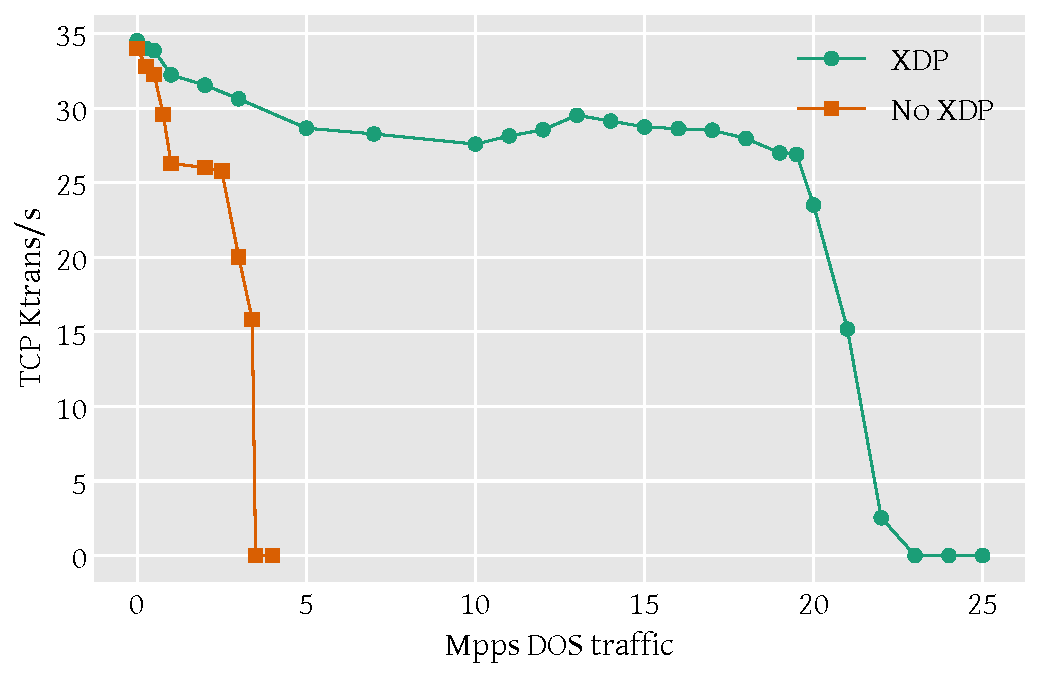
\includegraphics[width=\linewidth]{images/ddos-test.pdf}
\caption{\label{fig:ddos-results} DDoS protection performance. Number of TCP
  transactions per second as the level of attack traffic directed at the server
  increases.}
\end{figure}

We believe it is possible to generalise the mechanism that defers SKB creation,
to the point where this can be moved out of drivers entirely. The main thing
missing before we can achieve this, is a way to transfer the information from
different driver offloads (e.g., checksums, RX hashing, HW-marking) in a vendor
neutral and generic way. We have high hopes that the metadata work also
presented at LPC~\cite{xdp-metadata} will be a way to achieve this.


\subsection{Decoupling ndo\_xdp\_xmit resource allocation from XDP loading}
\label{sec:decoupling-ndo-xdp-xmit}

When XDP redirects a frame out another \texttt{net\_device}, then the
\texttt{ndo\_xdp\_xmit()} function of that device's driver is called. However,
enabling \texttt{ndo\_xdp\_xmit()} means a hardware TX queue needs to be
allocated per CPU core, which ties up resources, and so drivers don't enable
this by default. The problem is that there is currently no interface to enable
\texttt{ndo\_xdp\_xmit()} by itself; rather, it is enabled when an XDP program
is loaded. This leads to the current situation where a dummy XDP program needs
to be loaded on the device that is the target of an XDP redirect. This needs to
be done even if that device doesn't need to do any XDP ingress processing
itself, and if no XDP program is loaded on the target device, packets will just
be dropped silently.

Apart from being a bad user interface, this coupling of TX queue allocation to
XDP program loading is a waste of resources in the case where a device is
\emph{not} going to be a target of redirects. In the worst case this can make it
impossible to use XDP on systems with many cores (for instance, it was
discovered that the ixgbe driver cannot load XDP on systems with more than 96
CPU cores). But even on smaller systems, reserving hardware queues that are not
really needed is wasteful. For this reason, we propose that the enabling
\texttt{ndo\_xdp\_xmit()} is decoupled from the loading of XDP programs, and
that a better trigger mechanism be implemented. An obvious choice is to enable
the functionality when a device is first inserted into a \texttt{DEVMAP} to be
used in XDP\_REDIRECT, although this leaves the question of what to do with the
non-map variant of REDIRECT.

\subsection{Partial XDP support in drivers}
\label{sec:partial-xdp-support}

Not all drivers that support loading XDP programs actually support the full
feature set, and there is currently no way for userspace to discover what a
device actually supports. For instance, if a driver doesn't support
XDP\_REDIRECT, then it can only be detected at runtime by observing a WARN\_ONCE
kernel log message; and afterwards packets are silently dropped. This is
problematic for applications that want to use XDP where it is available, but
fall back to another mechanism when it is not. Suricata is an example of an
application that has experienced this problem.

Originally, the decision not to expose XDP feature bits was taken based on the
assumption that all drivers would implement the full feature set. However, the
question is if this is still a realistic goal, given that there are still only
three hardware drivers that implement XDP\_REDIRECT, and that some users are
happy with just XDP\_DROP and XDP\_TX support. For this reason, we would like to
bring up this discussion again.

% FIXME: Should we write something about how we propose to solve this?

\subsection{XDP egress hook}
\label{sec:xdp-egress-hook}

A limitation of the current design of XDP is that programs get no feedback if a
redirect to another device fails. Instead, the packet is just silently dropped,
and the only way to see why is by attaching to the right tracepoint. This is
especially problematic when forwarding packets from a fast device to a slower
one. And the way \texttt{XDP\_REDIRECT} is implemented, there is no way for the
XDP program to gain insight into the state of the device being forwarded
\emph{to}.

We believe that a possible fix for this is to add another eBPF hook at packet
egress from a device, i.e., at the latest possible time before a packet is put
into the device TX ring. At this point, it is possible for the driver to supply
information about the current state of the TX ring buffer (such as free space),
which the eBPF program can react appropriately to, for example by signalling
ingress XDP programs to send traffic another way if the TX ring is full, or by
implementing AQM-like reactions when TX ring pressure increases.

\section{Conclusion}
\label{sec:conclusion}

We have provided an overview of the current XDP-related work being discussed at
LPC '18, which includes production deployment reports, using XDP as a backend
for the P4 language, zero-copy to userspace with AF\_XDP, and the use of kernel
helpers to evolve the XDP feature set. We have also discussed some future
directions for XDP development which we believe will be beneficial to pursue.
These include NIC memory models and DMA mapping; moving SKB allocation out of
drivers; the resource allocation around ndo\_xdp\_xmit; whether it is still
realistic to aim for full support of all XDP features in all drivers; and the
possibility for adding an XDP egress hook.

It is our hope that this can serve as a useful overview, and as a catalyst for
discussion of the longer-term future for the XDP system as a whole.


\bibliographystyle{ACM-Reference-Format}
\bibliography{xdp-future}

\end{document}
